% !TEX root=../main.tex

\subsection{Extracting the selection efficiency} \label{sec:efficiencyPidExtraction}

Referring to \autoref{fig:efficiencyByCut} it is evident that the first selection cut, i.e. CRT-PMT matching, has no impact on the events.
For the present study, this is due to the type of events analysed, that include only neutrino candidate interactions, i.e. neither in-time nor out-of-time cosmics are simulated.
The second cut, Flash-match, has a very small effect: this has the same explanation as CRT-PMT cut, since no cosmic-ray interaction is generated for the presently used sample.
The first cut that introduces a reduction in the selected statistics is the requirement on the vertex position to lie inside the fiducial volume of the detector.
This is a request that is strongly dependent on the reconstruction performance; therefore, it is expected that an improved vertex reconstruction results in an overall improvement on the efficiency.
The following request that all particles are contained in the active volume of the detector is also strongly dependent on the reconstruction performance. Correct clustering of the hits and start-/end-point assignation is correlated with containment (if the true particles are contained, so should be the reconstructed ones). 
The last selection cuts concern the muon and proton identifications and the no-charged-pion and no-electromagnetic-shower requests. These have a large impact on the event selection efficiency, with a ${\sim}\SI{15}{\percent}$ loss in the identification of the proton, followed by the ${\sim}\SI{5}{\percent}$ loss due to the identification and rejection of charged pions and electromagnetic showers. The particle identification cuts, described in detail in \autoref{sec:dataSample_and_selection}, follows from cuts on variables that are direct consequence of the efficiency of Pandora reconstruction, such as the length requirements, the track and shower classification BDT score, the distance from the interaction vertex, and the particle hierarchy requirements, as well as variables that are heavily influeced by the calorimentric reconstruction performances, downstream of Pandora event reconstruction (see \autoref{sec:calorimetryAndCalibration}). Assuming the correlation between variables that depend on Pandora topological reconstruction quality and variables that depends on the calorimetric reconstruction effectiveness is small, it is possible to factorise their contribution to the final selection efficiency, assigning a ``reconstruction-related'' event selection efficiency to the former and a ``PID-related'' event selection efficiency to the latter, \begin{equation}
    \epsilon_\mathrm{event\ selection} = \epsilon_\mathrm{ev.\ sel.,\ reco.} \times \epsilon_\mathrm{ev.\ sel.,\ pid}. \label{eq:originalSelEfficiency}
\end{equation} 

Considering Eq. \eqref{eq:componentsEfficiency}, we can rewrite it, as \begin{equation}
    \begin{aligned}
        \epsilon &= 
        \epsilon_\mathrm{signal\ processing} \times 
        \epsilon_\mathrm{2D\ clusters} \times 
        \epsilon_\mathrm{vertex\ creation} \times 
        \epsilon_\mathrm{3D\ reconstruction} \times \\
        &\quad\quad\quad\times
        \epsilon_\mathrm{particle\ classification} \times 
        \epsilon_\mathrm{event\ selection,\ reco.} \times 
        \epsilon_\mathrm{event\ selection,\ pid}.
    \end{aligned} \label{eq:componentsEfficiencyPid}
\end{equation} We can make an additional assumption.
Since the term $\epsilon_\mathrm{event\ selection,\ reco.}$ is related to the reconstruction efficiency, it is reasonable to assume that each stage in the reconstruction chain will give its specific contribution to the overall value.
This hypothesis is supported, for example, by the observation that once the vertex reconstruction is cheated, the requirement that the vertex lie inside the TPC fiducial volume is automatically satisfied, as can be seen in \autoref{fig:efficiencyByCut}. In other words, the component of the selection efficiency associated with vertex containment is correlated with the success of correctly assigning the true interaction vertex. Taking this into account, we can rewrite Eq. \eqref{eq:componentsEfficiencyPid} as \begin{equation}
    \begin{aligned}
        \epsilon &= 
        \epsilon_\mathrm{signal\ processing} \times 
        \epsilon_\mathrm{2D\ clusters}' \times 
        \epsilon_\mathrm{vertex\ creation}' \times 
        \epsilon_\mathrm{3D\ reconstruction}' \times \\
        &\quad\quad\quad\times
        \epsilon_\mathrm{particle\ classification}' \times 
        % \epsilon_\mathrm{event\ selection,\ reco.} \times 
        \epsilon_\mathrm{ev.\ sel.,\ pid}
        = 
        \epsilon_\mathrm{sig.\ proc.} \times 
        \epsilon_\mathrm{reco.}' \times 
        \epsilon_\mathrm{ev.\ sel.,\ pid},
    \end{aligned} \label{eq:componentsEfficiencyPidNew}
\end{equation} where the prime symbol $'$ is added to highlight that the efficiencies listed here slightly differ from the ones above in Eq. \eqref{eq:componentsEfficiencyPid}. Following the same strategy outlined in Eq. \eqref{eq:componentsEfficiency}--\eqref{eq:stageEfficiencyPrePID}, we now obtain a new version of \begin{equation}
    \epsilon_\mathrm{particle\ class.} \times \qty(\frac{
    \epsilon_\mathrm{ev.\ sel., pid}^\mathrm{B}
    }{
    \epsilon_\mathrm{ev.\ sel., pid}^\mathrm{A}
    }) = \frac{
    \epsilon^\mathrm{B}
    }{
    \epsilon^\mathrm{A}
    }. 
\end{equation} where we dropped the prime symbol for simplicity. We can now invert the equation to extract the term we want to evaluate: \begin{equation}
    \epsilon_\mathrm{particle\ class.} = \frac{
    \epsilon^\mathrm{B}
    }{
    \epsilon^\mathrm{A}
    } \times \frac{
    \epsilon_\mathrm{ev.\ sel., pid}^\mathrm{A}
    }{
    \epsilon_\mathrm{ev.\ sel., pid}^\mathrm{B}
    }, \label{eq:stageEfficiencyPostPID}
\end{equation} It is clear that to do this we need a final ingredient, which is given by the impact of PID onto selection efficiency, i.e.,  $\epsilon_\mathrm{ev.\ sel.,\ pid}$. To extract such a parameter, we developed a modified event selection that allowed the effects of particle identification to be decoupled from the effects of the event reconstruction. In this modified event selection, all the cuts performed on variables that depend on the reconstruction performance are left unaltered, whereas the cuts that are dependent on the calorimetric particle identification are effectively bypassed considering the true particle labels. The requirements for this ``modified'' particle identification are detailed below.  

\noindent
To identify if a single muon is present in the interaction, the following cuts are applied: \begin{itemize}
    \item the particle should be tagged as a primary particle by Pandora,
    \item the conversion gap should be smaller than \SI{10}{\cm},
    \item the track/shower classification score should be greater than 0.5,
    \item the track length should be greater than \SI{50}{\cm},
    \item the label assigned via match with Monte Carlo information should correspond to a muon. 
\end{itemize}
For the protons in the interaction, the following cuts are applied: \begin{itemize}
    \item the particle should be tagged as a primary particle by Pandora,
    \item the conversion gap should be smaller than \SI{10}{\cm},
    \item the track/shower classification score should be greater than 0.4,
    \item the reconstructed deposited energy and the true kinetic energy should be greater than \SI{50}{\MeV},
    \item the label assigned via match with Monte Carlo information should correspond to a proton.
\end{itemize}
For pions, the selection is the same as for protons, with the sole difference of requiring the true label of a charged pion and a lower energy threshold of \SI{25}{\MeV}. 

\noindent
For electromagnetic showers, the following cuts are applied: \begin{itemize}
    \item the particle should be tagged as a primary particle by Pandora,
    \item the track/shower classification score should be smaller than 0.5,
    \item the reconstructed deposited energy and the true kinetic energy should be greater than \SI{25}{\MeV},
    \item the label assigned via match with Monte Carlo information should correspond to an electron or a photon. 
\end{itemize} 


Using this modified event selection, we extract again the efficiencies as a function of cheated stages and selection cuts (see \autoref{fig:efficiencyNoNu}). \autoref{fig:CCNp_efficiencyNoNu_cheatingPid} shows the efficiency for the same configurations (see \autoref{tab:configurations}) with the modified event selection. 

\begin{figure}
    \centering
    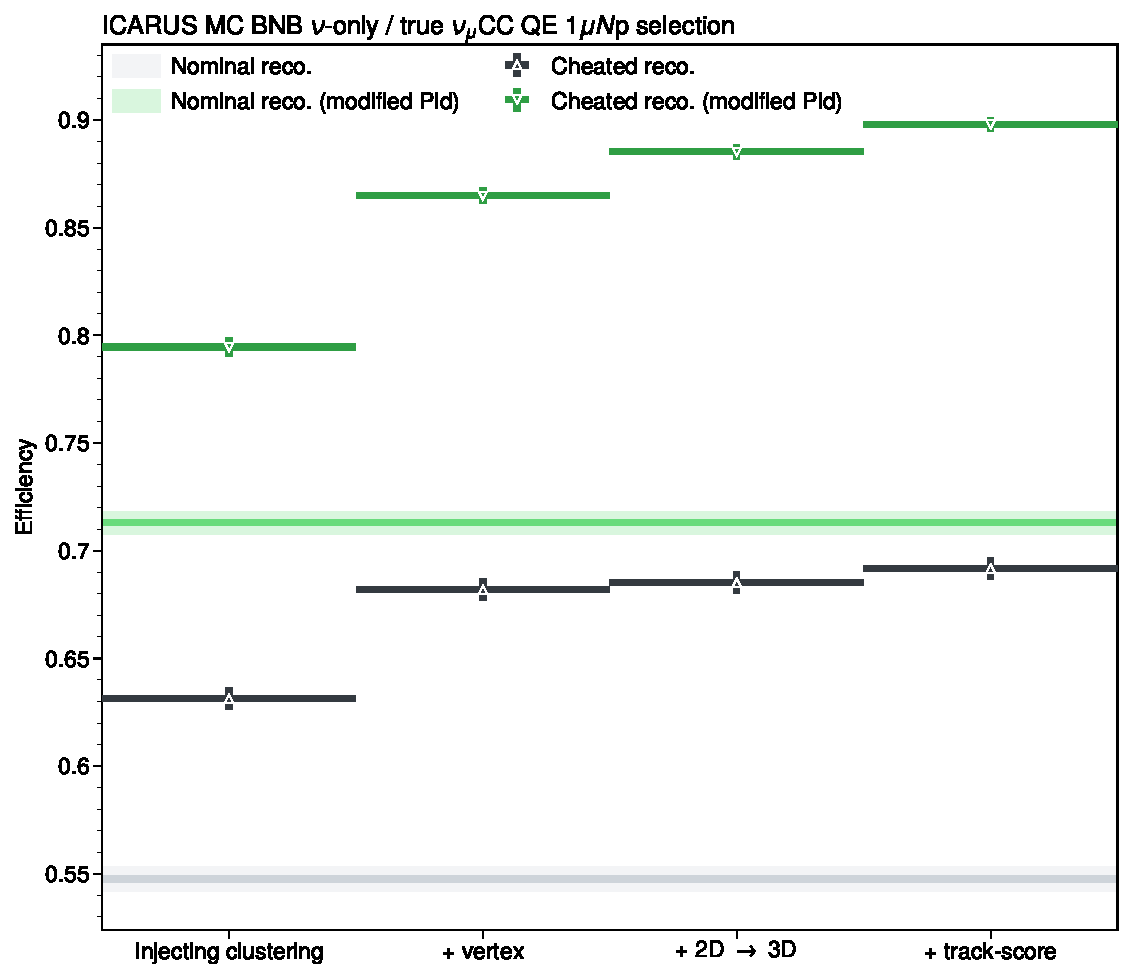
\includegraphics[width=0.85\linewidth]{pandora/chapter_4/CCNp_efficiencyNoNu_cheatingPid.pdf}
    \caption[Evaluation of the reconstruction and selection efficiency for different configurations with the modified event selection]{Evaluation of the event reconstruction and selection efficiency for all the configurations listed in \autoref{tab:configurations}. Both the event selection with the nominal particle identification (black markers) and the event selection with the modified particle identification (green markers) are shown. }
    \label{fig:CCNp_efficiencyNoNu_cheatingPid}
\end{figure}

% Extracting the efficiency here
For this modified event selection we can assume that the overall efficiency that accounts both for reconstruction, PID and selection is \begin{equation}
    \epsilon^\mathrm{mod.\ selection} = \epsilon_\mathrm{sig.\ proc.} \times 
        \epsilon_\mathrm{reco.} \times 
        \epsilon_\mathrm{ev.\ sel.,\ pid}^\mathrm{mod.\ selection}. 
        \label{eq:modifiedPidEfficiency}
\end{equation} This modified event selection does not rely on the performance of the PID, using the true underlying MC label to uniquely identify reconstructed particle species. Therefore we assumed that  $\epsilon_\mathrm{ev.\ sel.,\ pid}^\mathrm{mod.\ selection}\simeq1$, since no particle misidentification inefficiencies related to PID are possible. We exploit this simplification, and comparing Eq. \eqref{eq:modifiedPidEfficiency} and \eqref{eq:componentsEfficiencyPidNew}, we can extract the efficiency of the particle identification stage for each configuration of \autoref{tab:configurations}. The ratio of these two equations leads to \begin{equation}
    \frac{
    \epsilon^{\mathrm{mod.\ selection,}\ c}
    }{
    \epsilon^{c}
    } = \frac{
    \epsilon_\mathrm{sig.\ proc.} \times 
    \epsilon_\mathrm{reco.} \times 
    \epsilon_\mathrm{ev.\ sel.,\ pid}^{\mathrm{mod.\ selection,}\ c}
    }{
    \epsilon_\mathrm{sig.\ proc.} \times 
    \epsilon_\mathrm{reco.} \times 
    \epsilon_\mathrm{ev.\ sel.,\ pid}^c
    } = \frac1{\epsilon_\mathrm{ev.\ sel.,\ pid}^c} \label{eq:tmpEq20}
\end{equation} for each configuration $c$. By inverting Eq. \eqref{eq:tmpEq20} we can estimate the contribution of particle identification, and thus calorimetric reconstruction, to the overall selection efficiency. \begin{equation}
    \epsilon_\mathrm{ev.\ sel.,\ pid}^c = \frac{
    \epsilon^{c}
    }{
    \epsilon^{\mathrm{mod.\ selection,}\ c}
    }. \label{eq:pidComputation}
\end{equation} The particle identification efficiencies extracted are reported in \autoref{tab:pidEfficiencyPerConfiguration}. 

\begin{table}[]
    \centering
    \caption[Particle identification efficiency for all configurations]{For each configuration the corresponding efficiency is shown, using both the nominal event selection and the modified event selection described in \autoref{sec:efficiencyPidExtraction}. The third column is the resulting efficiency of the particle identification step.  Further details on the evaluation of the listed parameters are provided in the text.}
    \label{tab:pidEfficiencyPerConfiguration}
    \begin{tabular}{lp{3.5cm}ccc}
        \hline
         Id. & Configuration name & $\epsilon$ & $\epsilon^\mathrm{mod.\ selection}$ & $\epsilon_\mathrm{ev.\ sel.,\ pid}$ \\
         & & (see Eq. \ref{eq:originalSelEfficiency}) & (see Eq. \ref{eq:modifiedPidEfficiency}) & (see Eq. \ref{eq:pidComputation})\\ 
         \hline
         A & Fully cheated & \SI{69.2(5)}{\percent} & \SI{89.78(33)}{\percent} & \SI{77.1(6)}{\percent} \\
         B & Cheated up to the particle classification algorithm & \SI{68.5(5)}{\percent} & \SI{88.52(35)}{\percent} & \SI{77.4(6)}{\percent} \\
         C & Cheated up to the particle three-dimensional reconstruction algorithm & \SI{68.2(5)}{\percent} & \SI{86.5(4)}{\percent} & \SI{78.8(7)}{\percent} \\
         D & Cheated up to the vertex reconstruction & \SI{63.1(5)}{\percent} & \SI{79.5(4)}{\percent} & \SI{79.4(8)}{\percent} \\
         E & Nominal & \SI{54.8(5)}{\percent} & \SI{71.3(5)}{\percent} & \SI{76.8(9)}{\percent} \\
         \hline
    \end{tabular}
\end{table}

By replacing the PID efficiency values extracted thanks to the modified selection in Eq. \eqref{eq:stageEfficiencyPostPID}, we can derive an estimate for the efficiency of each stage of the reconstruction. This leads to the following results \begin{equation}
    \begin{aligned}
        \epsilon_\mathrm{reco.} =&\
        \epsilon_\mathrm{2D\ clusters} &\times&\ 
        \epsilon_\mathrm{vertex\ creation} &\times&\ 
        \epsilon_\mathrm{3D\ reco.} &\times&\ 
        \epsilon_\mathrm{particle\ class.} =\\  
        =&\ \SI{89.7(1.8)}{\percent} &\times&\ 
        \SI{91.9(1.6)}{\percent} &\times&\ 
        \SI{97.7(1.6)}{\percent} &\times&\ 
        \SI{98.6(1.5)}{\percent}
    \end{aligned}\label{eq:results}
\end{equation}

These findings should be interpreted with caution. Firstly, they are obtained targeting a specific event topology. Therefore, it is reasonable to assume that a different event topology would yield significantly different results. As explicitly stated throughout the text, numerous assumptions and approximations have been made to obtain these results. All correlations between the various algorithms involved in Pandora reconstruction chain are assumed to be minimal. Additionally, to obtain the selection efficiencies, most of the variables involved in the event selection cuts are assumed to be uncorrelated. These assumptions hold true to a certain extent. 

However, as discussed in the subsequent section, an independent test on the vertex reconstruction was conducted. The results from this independent test, which are in good agreement with the results in Eq. \eqref{eq:results}, suggest that the starting point hypothesis is reasonable. 